\chapter{Data acquisition for CHIPS} %%%%%%%%%%%%%%%%%%%%%%%%%%%%%%%%%%%%%%%%%%%%%%%%%%%%%%%%%%%%%
\label{chap:daq} %%%%%%%%%%%%%%%%%%%%%%%%%%%%%%%%%%%%%%%%%%%%%%%%%%%%%%%%%%%%%%%%%%%%%%%%%%%%%%%%%

\begin{comment} % PLAN %%%%%%%%%%%%%%%%%%%%%%%%%%%%%%%%%%%%%%%%%%%%%%%%%%%%%%%%%%%%%%%%%%%%%%%%%%%
- What makes this implementation special
- Limited resource, but brilliant capabilities
- Use existing software when possible

- Need to talk about what is novel, new and exciting!
- Not so much about the hardcore electronics details, more high level
- FINITE STATE MACHINE!!!

HARDWARE
- The White Rabbit timing system
- Km3NET hardware
- Madison hardware (novel)
- Combined systems

SOFTWARE
- The beam spill
- Hit acquisition and handling
- Detector and data quality monitoring
\end{comment}

The primary task of any Data Acquisition (DAQ) system is the processing of low-level signals
measuring real-world physics and their transfer to permanent storage for further analysis.
Commonly, this procedure also includes decision making as to whether the signal is deemed
interesting enough to record, known as a \emph{trigger}. DAQ systems can quickly become incredibly
complex, especially when considering that it must be done in an efficient and resilient manner for
vast amounts of data in real-time, while also providing detector control and monitoring.

In the context of the \chips project, the DAQ system records all PMT hits, timestamps them using a
common clock, and then transfers them out of the detector to a central processing node. This node
then applies a trigger to only select hits that fall within the interesting beam spill. All
selected hits are then be sliced into \emph{events} and moved to permanent storage for further
analysis. Alongside these processes, the DAQ also configures all the PMTs within the detector and
provides data quality and detector component monitoring.

Although relatively simple when compared to the complex and time-pressured DAQ systems of the LHC
experiments, the DAQ system developed for the \chips project introduces novel approaches to solve
the unique constraints of \chips. Namely, deployment within a body of water and a limited budget.
In this chapter, the DAQ implementation for \chips as applied to the \chipsfive prototype detector
module is described.

\section{White Rabbit timing} %%%%%%%%%%%%%%%%%%%%%%%%%%%%%%%%%%%%%%%%%%%%%%%%%%%%%%%%%%%%%%%%%%%%
\label{sec:daq_timing} %%%%%%%%%%%%%%%%%%%%%%%%%%%%%%%%%%%%%%%%%%%%%%%%%%%%%%%%%%%%%%%%%%%%%%%%%%%

To ensure PMT hit times are synchronised throughout \chips detectors, a common clock must be
shared across all timestamping electronics. For this purpose \chips employs a \emph{White Rabbit}
(WR) network~\cite{lipinski2011}. Initially developed at CERN, the open-source WR project provides
an ethernet-based time distribution network with sub-nanosecond synchronisation accuracy between
nodes. By using a two-way exchange of WR messages, precise adjustment of individual clock phases
and offsets is possible across thousands of nodes, separated by tens of kilometres. All of this is
achieved in parallel with a standard data transfer network capable of \unit{1}{\mathrm{Gb}}
speeds.

All nodes are synchronised to the clock of a \emph{GrandMaster} node which is typically a WR
\emph{switch}, the most common WR hardware component. This switch receives as input a Pulse Per
Second (PPS) and \unit{10}{\mathrm{MHz}} signal from a GPS disciplined oscillator. When used in
conjunction with a Network Time Protocol (NTP) server connection, these inputs allow for the WR
network to be synchronised to International Atomic Time (TAI). This is particularly important for
\chips detector modules which require synchronisation to accelerator beam clocks (such as the
Fermilab Main Injector clock in the \chipsfive case) in order to determine the arrival of beam
spills accurately.

WR hardware is commercially available from many vendors. Within \chipsfive two WR devices are used
for time synchronisation and data transfer, both shown in Fig.~\ref{fig:wr_electronics}. Firstly,
a compact version of the standard WR switch~\cite{wrswitch2020}, specially developed for the
\chips project at Nikhef~\cite{wrchromium2020}. Secondly, a WR Lite Embedded Node (LEN) from Seven
Solutions~\cite{wrlen2020}. All WR components within \chipsfive are connected using
\unit{1}{\mathrm{Gb}} bi-directional optical fibre connections using the \unit{1310}{\mathrm{nm}}
and \unit{1550}{\mathrm{nm}} wavelengths via Small Form-Factor Pluggable Transceivers (SFPs).

\begin{figure} % WHITE-RABBIT COMPONENTS DIAGRAM %
    \centering
    \subcaptionbox{White Rabbit switch}{%
        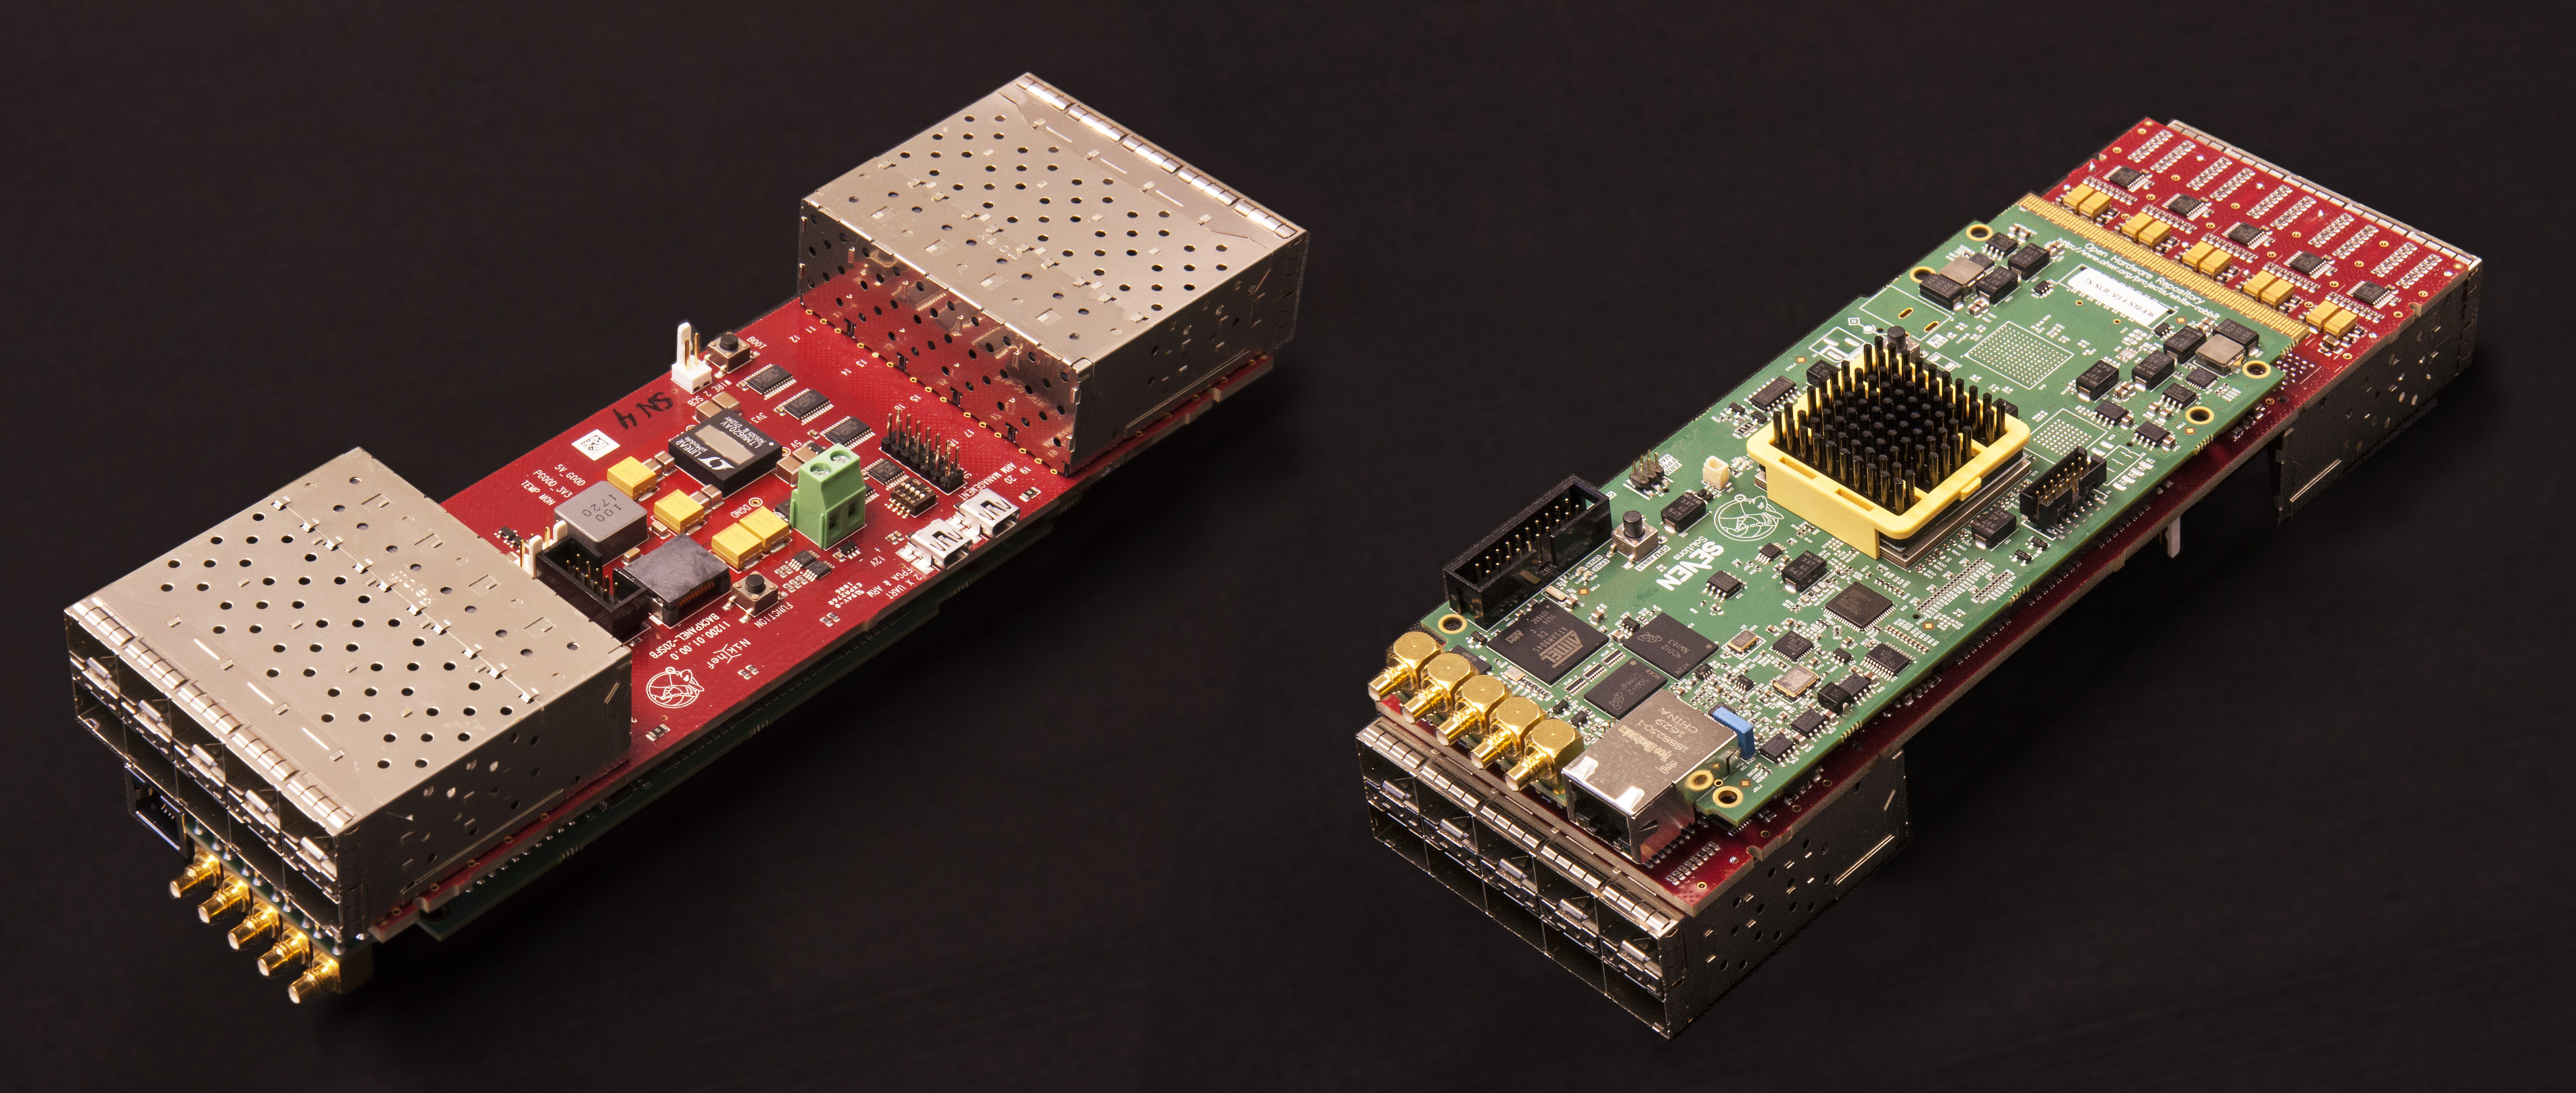
\includegraphics[height=6cm]{diagrams/5-daq/wr_switch.jpg}%
    }
    \quad
    \subcaptionbox{White Rabbit LEN}{%
        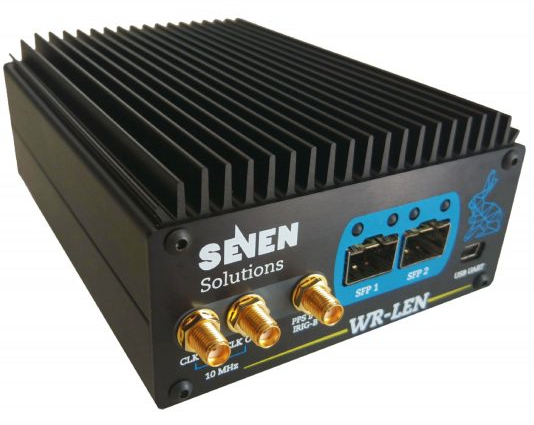
\includegraphics[height=6cm]{diagrams/5-daq/wr_len.jpg}%
    }
    \caption[Pictures of the White Rabbit timing hardware used within \chipsfive.]
    {Pictures of the White Rabbit timing hardware used within \chipsfive. The compact White rabbit
        switch specially designed for \chips is shown in (a), while the White Rabbit Lite Embedded
        Node (LEN) from Seven Solutions is shown in (b).}
    \label{fig:wr_electronics}
\end{figure}

Fig.~\ref{fig:sync} shows the resulting WR synchronised PPS clock signals from two WR switches
used within \chipsfive and separated by \unit{500}{\mathrm{m}} of fibre. With the vertical ticks
representing nanoseconds, the sub-nanosecond time synchronisation accuracy is observed.

\begin{figure} % WHITE-RABBIT SYNC DIAGRAM %
    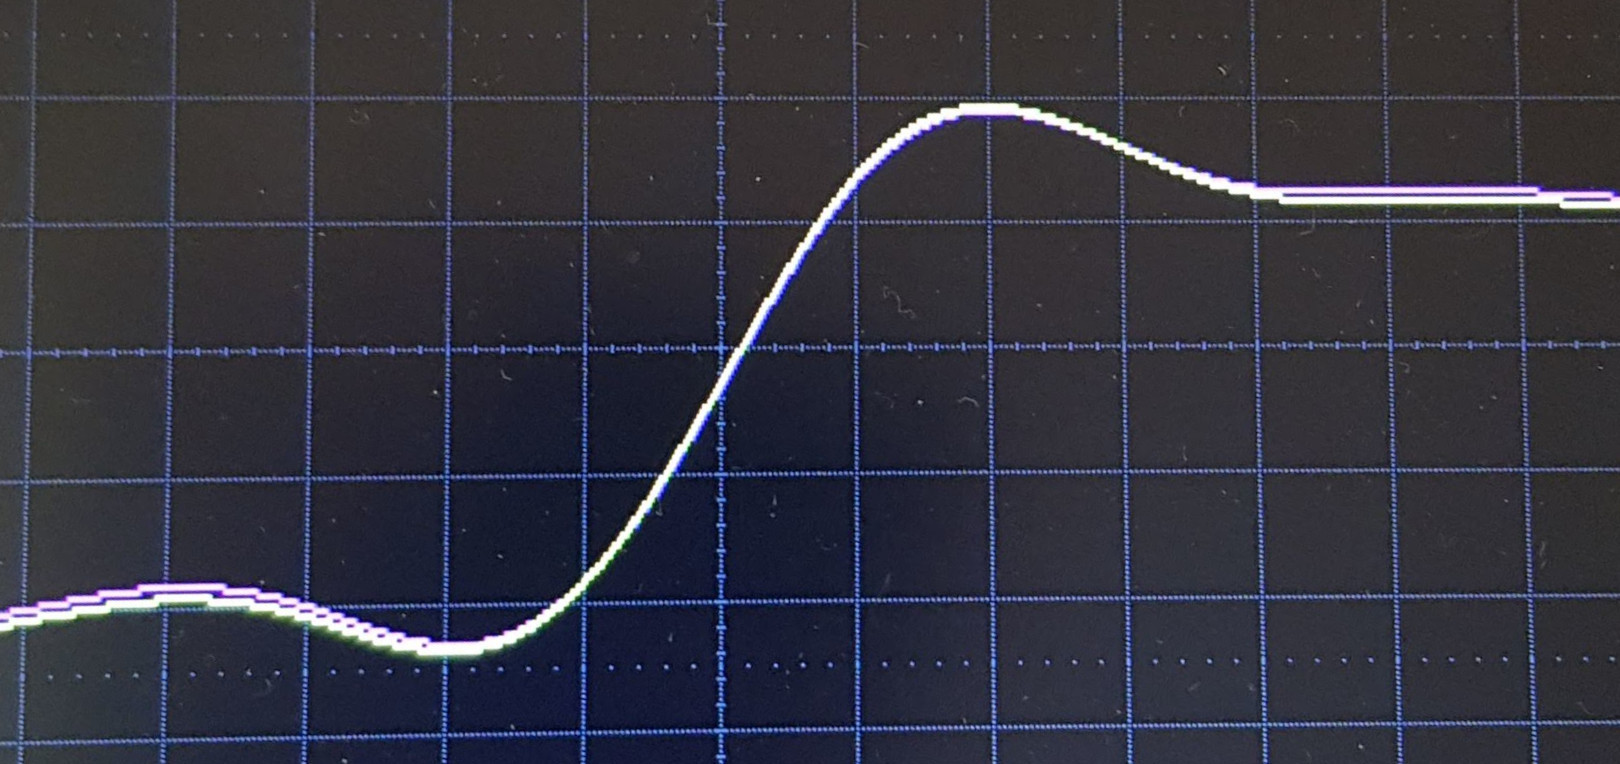
\includegraphics[width=0.7\textwidth]{diagrams/5-daq/sync.jpg}
    \caption[Picture of White Rabbit timing synchronisation seen in \chips.]
    {Picture of an oscilloscope measuring the PPS output signal of two WR switches shown in pink
        and yellow at either end of a \unit{500}{\mathrm{m}} long optical fibre. The vertical
        ticks are in nanoseconds showing the sub-nanosecond synchronisation possible with the WR
        timing network.}
    \label{fig:sync}
\end{figure}

\section{Hardware} %%%%%%%%%%%%%%%%%%%%%%%%%%%%%%%%%%%%%%%%%%%%%%%%%%%%%%%%%%%%%%%%%%%%%%%%%%%%%%%
\label{sec:daq_hard} %%%%%%%%%%%%%%%%%%%%%%%%%%%%%%%%%%%%%%%%%%%%%%%%%%%%%%%%%%%%%%%%%%%%%%%%%%%%%

The primary task of the DAQ system is to transfer timestamped


Power and data flow

Will discuss Nikhef and Madison separately for for clarity.

- Start from the bottom and work our way up!
- The task is to take TOT recorded hits, that are timestamped using the white-rabbit stuff and get
them to storage at Fermilab, all sorted, without losses, in a timely manner.
- Talk about general time resolution of the PMTs etc in the context of the overall time resolution
with the white rabbit.

Regardless of being either Nikhef or Madison all PMT electronics records the time-over-threshold
for hits. Instead of the more common ADC, this is mainly because the electronics is simpler and
therefore cheaper.

\begin{figure} % TOT DIAGRAM DIAGRAM %
    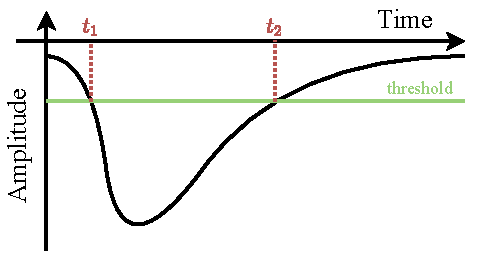
\includegraphics[width=0.7\textwidth]{diagrams/5-daq/tot.pdf}
    \caption[Illustrative diagram showing how time-over-threshold is measured.]
    {Illustrative diagram showing how time-over-threshold is measured. As soon as the rising edge
        of the charge pulse from a photon cascade passes a threshold a time is recorded, when the
        falling edge passes the threshold again a second time is recorded. The difference in time
        is output by the electronics as the time-over-threshold value.}
    \label{fig:tot}
\end{figure}

\begin{figure} % DAQ DIAGRAM %
    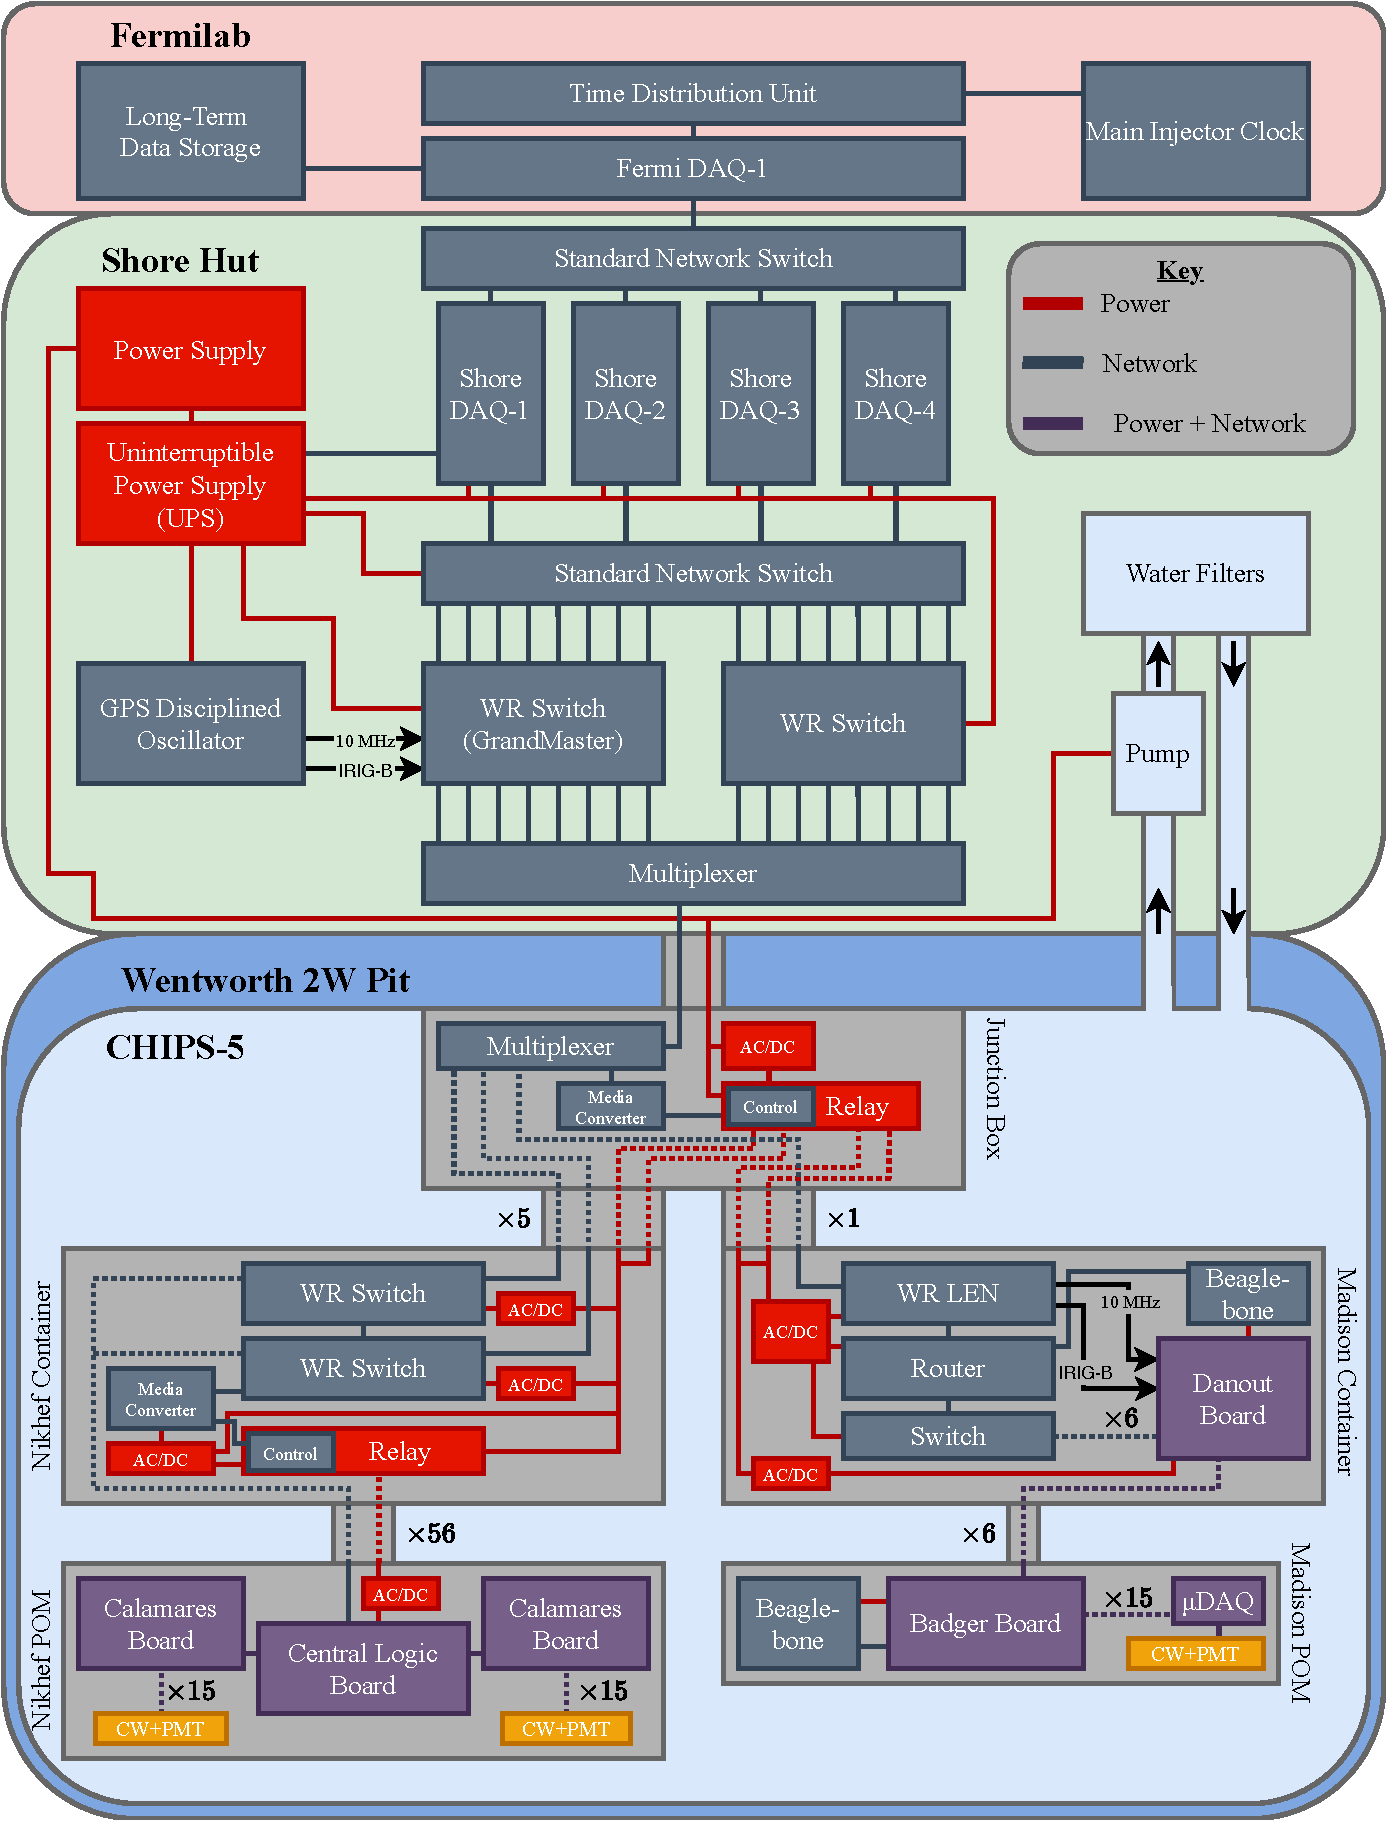
\includegraphics[width=\textwidth]{diagrams/5-daq/daq.pdf}
    \caption[Diagram of the \chipsfive data acquisition and power distribution system.]
    {Diagram of the \chipsfive DAQ and power distribution system.}
    \label{fig:daq}
\end{figure}

\subsection{Km3NET hardware} %%%%%%%%%%%%%%%%%%%%%%%%%%%%%%%%%%%%%%%%%%%%%%%%%%%%%%%%%%%%%%%%%%%%%
\label{sec:daq_hard_km3net} %%%%%%%%%%%%%%%%%%%%%%%%%%%%%%%%%%%%%%%%%%%%%%%%%%%%%%%%%%%%%%%%%%%%%%

- km3net daq ref in~\cite{biagi2015, adrian2016, eijk2015}

Starting from the lowest level (nearest the PMTs) going upwards the DAQ system is as follows. For
Nikhef planes the electronics box contains a Central Logic Board developed for KM3NeT which has an
onboard White-Rabbit controller, so the CLB itself contains a synchronised clock for timestamping
hits. PMT are attached to two calimares boards directly attached to the CLB via standard Category
5 cables using RJ45 connectors. The CLB receives a single fibre input and a direct power supply,
with a power supply

Multiple CLBs (POMs) are connected to a single Nikfef container, for which there are only five
within chipsfive. Each container, contains two White Rabbit switches for networking (two to
provide enough ports) and a relay board for controlling the power to all attached POMs. A media
converter converts a fibre connection to a standard copper cable connection to control the relay,
which is a network device. Both switches are also reachable on the network mainly for monitoring.
2 ac/ds converters provide power for each of the switches while a third powers the relay control
electronics and media converter. The relay outputs are connected directly to the input AC supply.

\begin{figure} % NIKHEF PLANE DIAGRAM %
    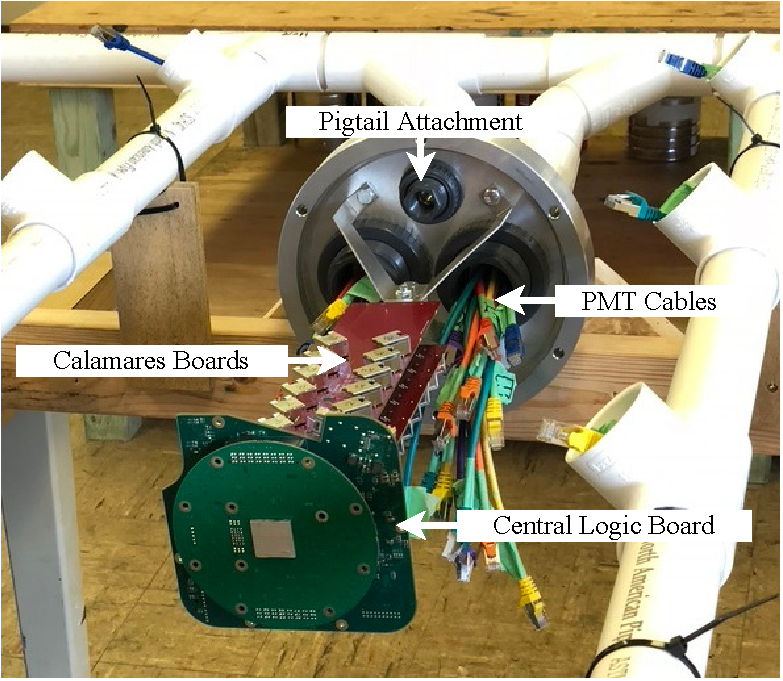
\includegraphics[width=0.8\textwidth]{diagrams/5-daq/nikhef_plane.pdf}
    \caption[nikhef plane short]
    {nikhef plane long}
    \label{fig:nikhef_plane}
\end{figure}

\subsection{Madison hardware} %%%%%%%%%%%%%%%%%%%%%%%%%%%%%%%%%%%%%%%%%%%%%%%%%%%%%%%%%%%%%%%%%%%%
\label{sec:daq_hard_madison} %%%%%%%%%%%%%%%%%%%%%%%%%%%%%%%%%%%%%%%%%%%%%%%%%%%%%%%%%%%%%%%%%%%%%

- Daan short ref in~\cite{eijk2018}
- Beaglebone ref in~\cite{beagle2020}

- THIS IS WHAT ALL FUTURE CHIPS DETECTOR SHOULD USE FULLY!!!
- This is the novel stuff that is much cheaper!

Each individual Madison R6091 PMT has an attached Cockroft Walton board and also a microDAQ, this
is a small microcontroller, that allows for all signal processing and timestamping to occur
directly at the PMT level unlike in the Nikhef case where it is done on the CLB. Each microDAQ
receives power, a half-duplex network connection and the two signals required for timestamping the
PPs and the 10Mhz. The Badger Board is a simple routing and fanout board to route the higher level
PPS and 10MhZ signals to each microDAQ while also providing them all with power. It also has an
mesinine beaglebone attached that provdes the actual on board logic. As the beaglebone is a full
linux machine at a low level lots of processing can occur close to the PMTs. It controls the power
and networking on the microDAQ, receives their hits before forwarding further up the chain.

The madison box contains what is shown in fig, it has a WR-LEN which is synchronised to the rest
of the WR network and outputs its PPS and 10MgHz singlas to the Danout board which is another
fanout, routing board for power, networking and the two signals, liek the badger board it has a
meanine beaglebone for logic which is connected to the netowkr and controls the powering of each
prt. A switch connection is made to each output port in order to connect each POM to the network.
THe router allows for the forwarding of traffic after the WR connectiong to the WR. This is done
via port forwarding to keep the Madision stuff as  a separate network.

GET THE COSTS OF THE WHOLE MADISON VS NIKHEF SYSTEM PER PLANE

\begin{figure} % MADISON BOX DIAGRAM %
    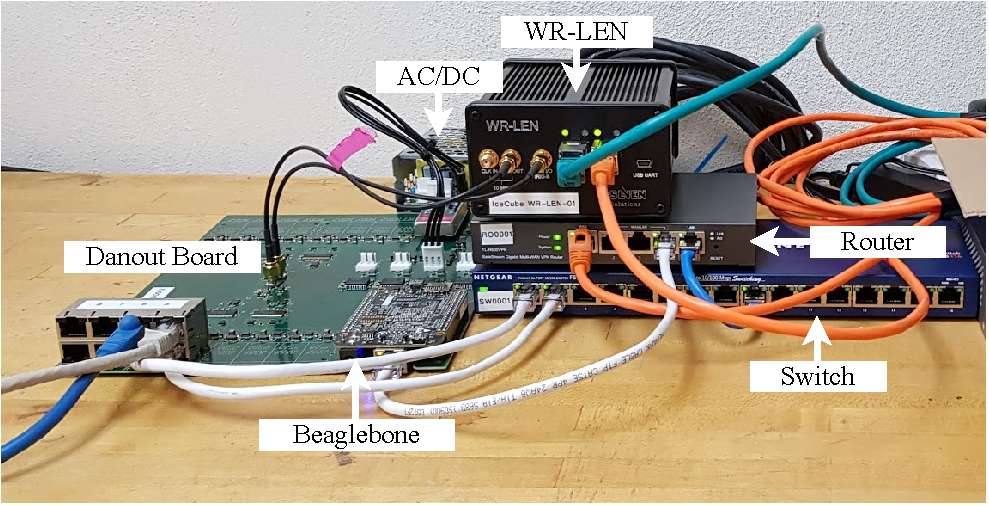
\includegraphics[width=\textwidth]{diagrams/5-daq/madison_box.pdf}
    \caption[madison box short]
    {madison box long}
    \label{fig:madison_box}
\end{figure}

\begin{figure} % MADISON PLANE DIAGRAM %
    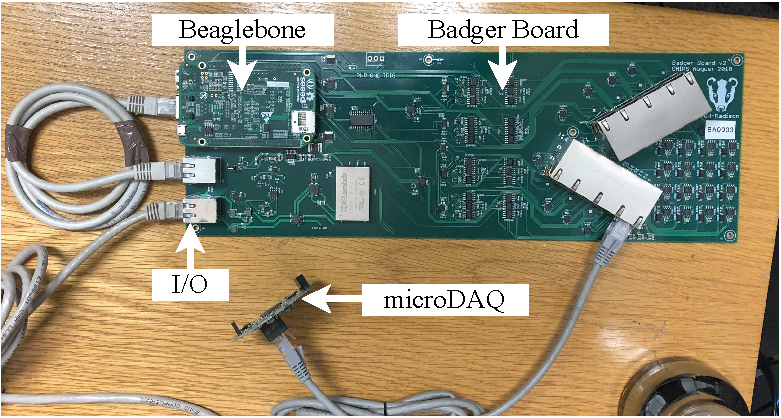
\includegraphics[width=0.8\textwidth]{diagrams/5-daq/madison_plane.pdf}
    \caption[madison plane short]
    {madison plane long}

    \label{fig:madison_plane}
\end{figure}

\subsection{Combined systems} %%%%%%%%%%%%%%%%%%%%%%%%%%%%%%%%%%%%%%%%%%%%%%%%%%%%%%%%%%%%%%%%%%%%
\label{sec:daq_hard_combined} %%%%%%%%%%%%%%%%%%%%%%%%%%%%%%%%%%%%%%%%%%%%%%%%%%%%%%%%%%%%%%%%%%%%

- Multiplexer allows for 16 different channels using wavelengths between 1310nm and 1550nm with
corresponding SFPs (Small Form-Factor Pluggable Transceiver)

The Junction box contains connections to each container and their power supply relays. The two
input power connections from shore are distributed to via two copper plates to all the relay
connections throughout the box. Two standard network contolled logic relays control "trip" gates
that stop the power supply to any/ section of the detector is a power surge is detected. THis is
espcecially important for CHIPS given the water that is everywher :p. One relay controls a pusing
and one just opens the channels. The trip gates are opening via a short pulse of current. Tye
multipleer contains 18 channels each a different wavelenght of light allowing a huge volume of
data to be sent up a single fibre to shore. Eahc WR swithc or WR LEN in the madison case has the
corresponding receiver SFP as the ones o shore.

Within the shore hut all netwoking comes in through the multiplexer and is split back out into its
individual wavelenght channels via the multiplexer these go into multiple ports on two white
rabbit switches. This is mainly for data flow such that each can be segmented via a VLAN with the
coresponding ports on the oppsitie side and then the higher level standard networking switch to
provide DO THE CALCULATION HERE lots of data bandwidth up to the main DAQ machines. One of the WR
sitches is the GrandMaster for the WR network and recievs the PPS and 10MhZ input from the GPs
disciplines ocillator anwhich is connected to a GPS antenna to receive its signals. Again both
switches are also on the DAQ network for monitoring and control.

The standard switch acts as the switch for condensing traffic onto single 10Gb connections to each
individual DAQ machine. This is also on the netwokr via a control port for monitoring. Only a
single DAQ machine is used for data taking which another is used for monitoring and control as
etailed inSection... The standard network switch is also connected to the wider CHIPS network at
the pit the polymet building and then the wider internet for data transfer to fermilab!

\begin{figure} % FULL SETUP DIAGRAM %
    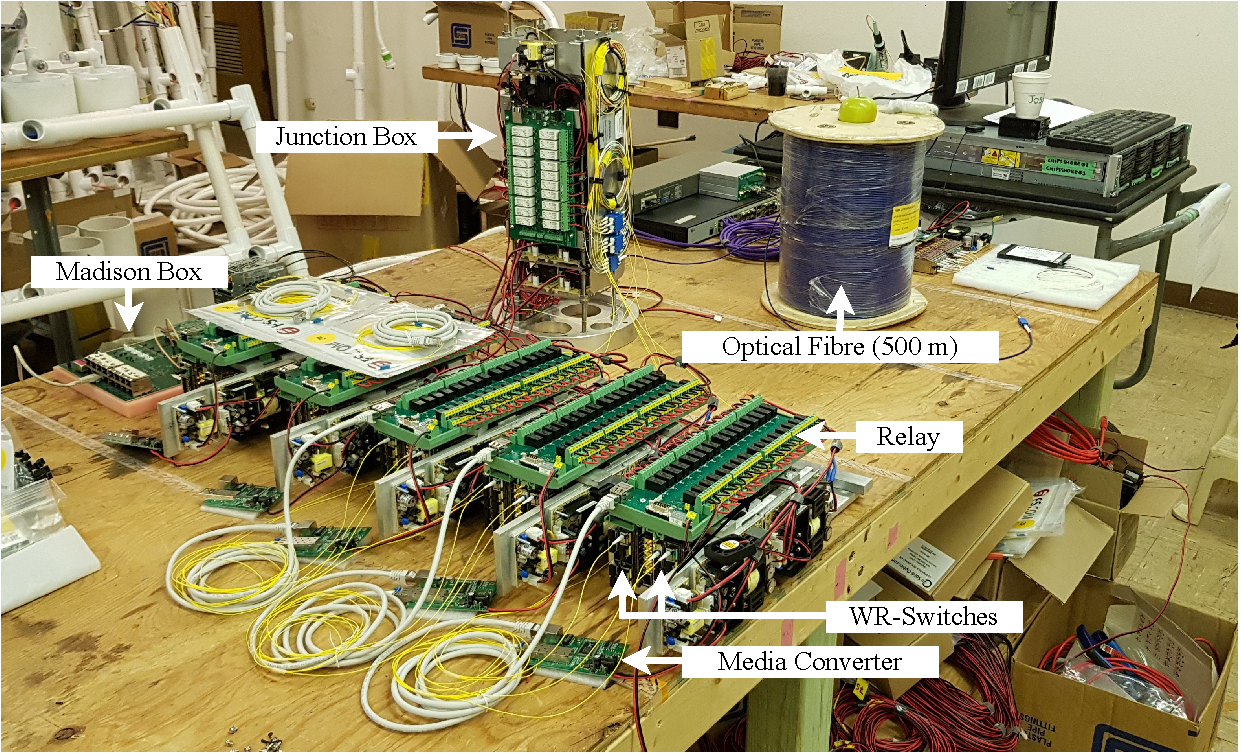
\includegraphics[width=\textwidth]{diagrams/5-daq/full_setup.pdf}
    %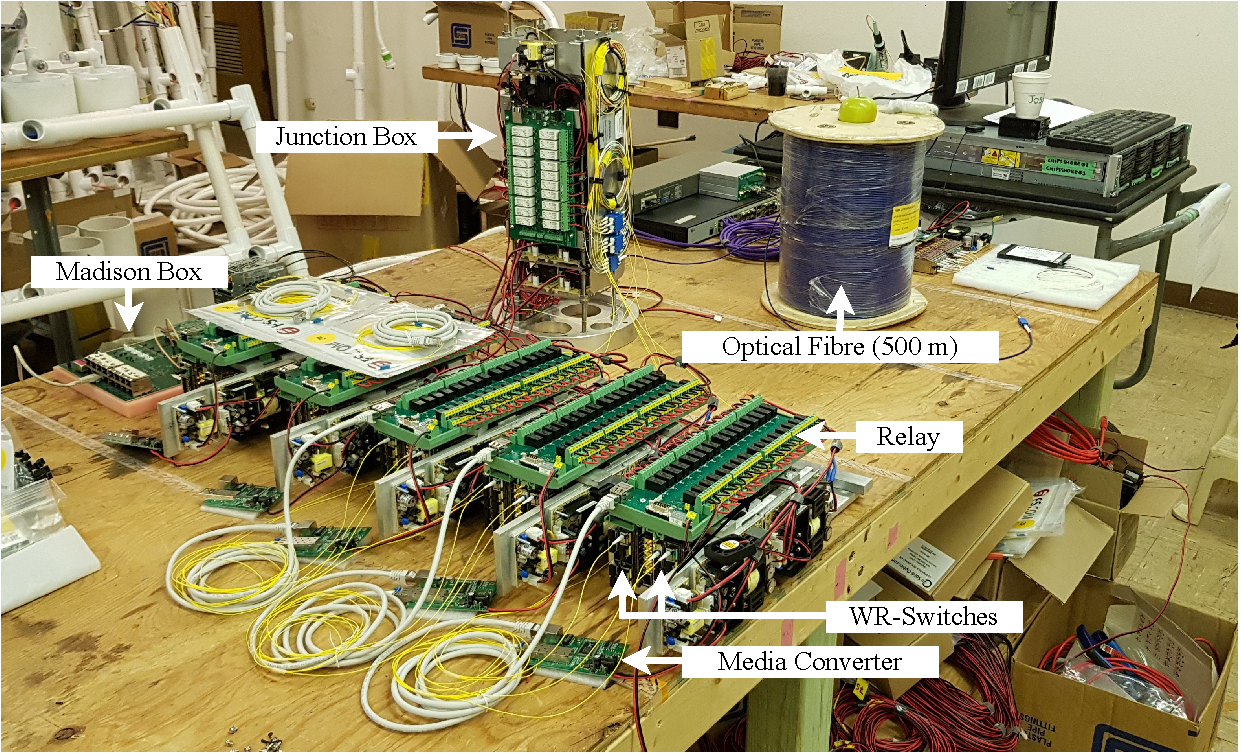
\includegraphics[angle=90,origin=c,width=0.8\textwidth]{diagrams/5-daq/full_setup.pdf}
    \caption[full set up short]
    {Picture of the full \chipsfive DAQ system}
    \label{fig:full_setup}
\end{figure}

\begin{figure} % MANIFOLD DIAGRAM %
    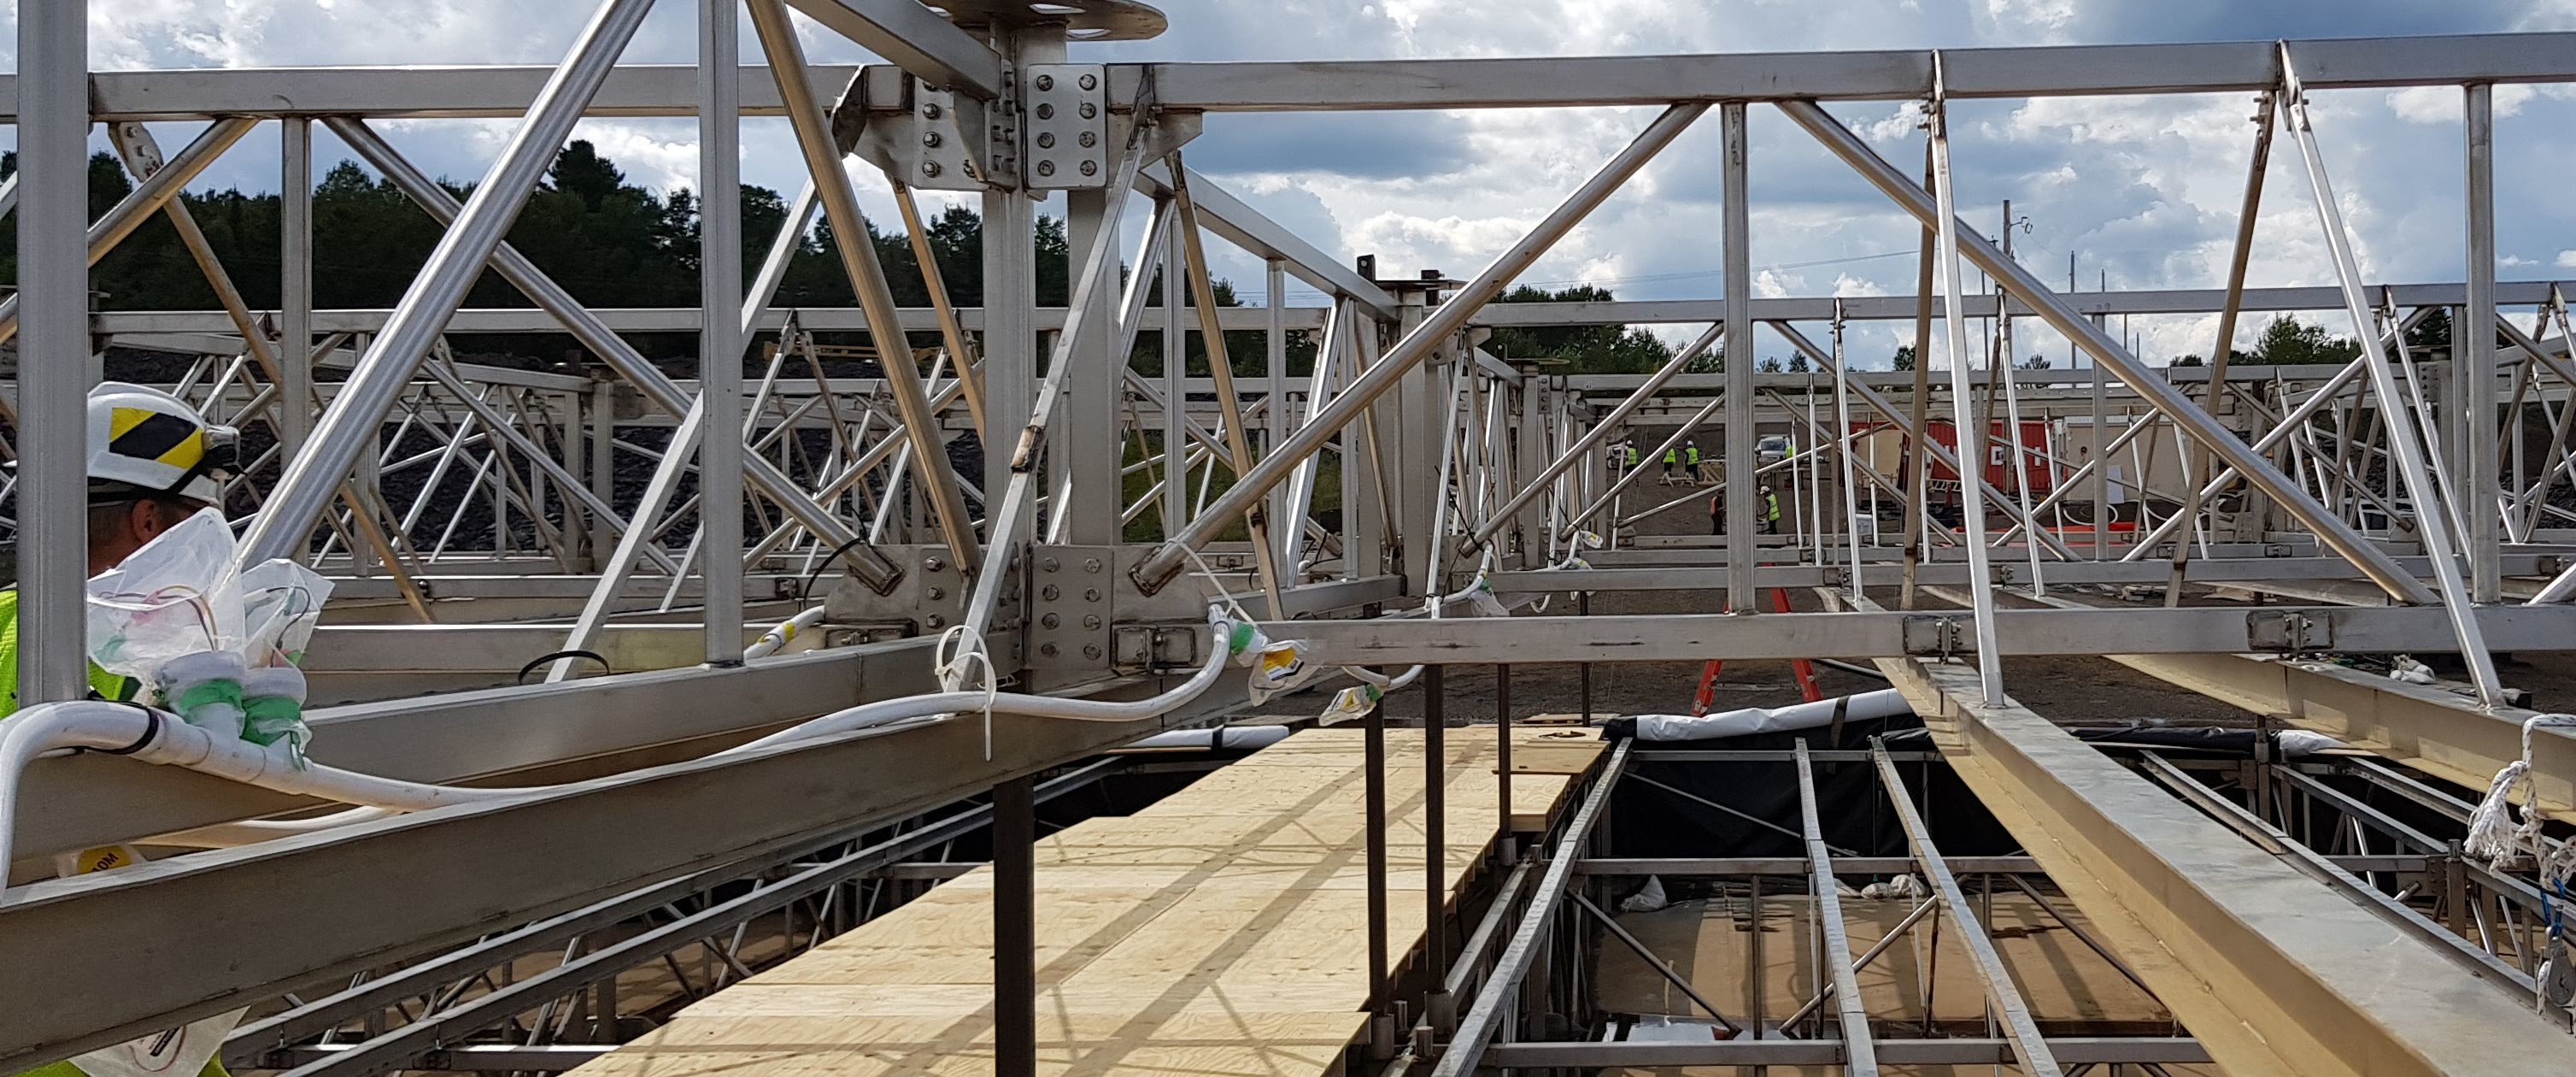
\includegraphics[width=\textwidth]{diagrams/5-daq/manifold.jpg}
    \caption[manifold short]
    {manifold long}
    \label{fig:manifold}
\end{figure}

\begin{figure} % WHITE-RABBIT GM SETUP DIAGRAM %
    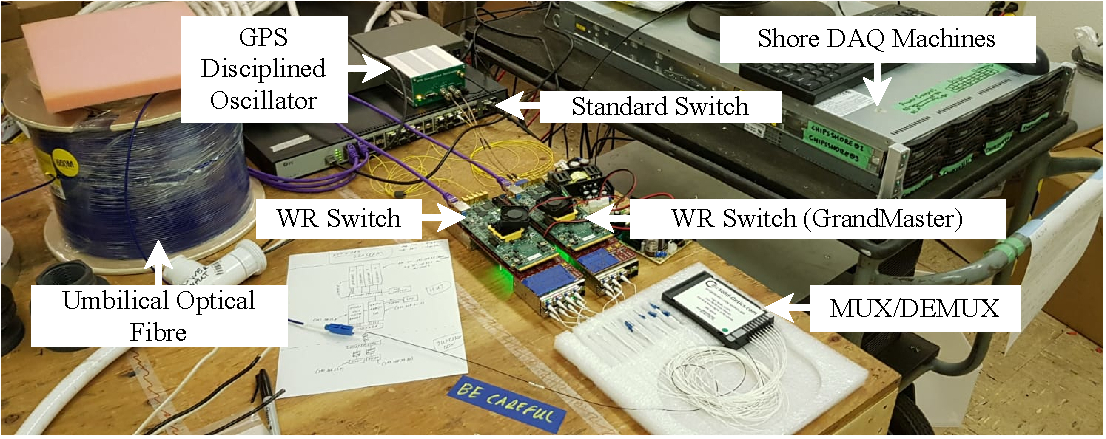
\includegraphics[width=\textwidth]{diagrams/5-daq/hut_daq.pdf}
    \caption[hut daq short]
    {hut daq long}
    \label{fig:hut_daq}
\end{figure}

\section{Data flow and software} %%%%%%%%%%%%%%%%%%%%%%%%%%%%%%%%%%%%%%%%%%%%%%%%%%%%%%%%%%%%%%%%%
\label{sec:daq_soft} %%%%%%%%%%%%%%%%%%%%%%%%%%%%%%%%%%%%%%%%%%%%%%%%%%%%%%%%%%%%%%%%%%%%%%%%%%%%%

DIAGRAM: Software diagram + finite state machine

- Separated into slow-control, data collection, and

- Need to get across what makes this DAQ implementation special and novel, what are the
interesting unique bits of it? Limited resources but great performance! Use of existing hardware
and software! Modern approaches to doing things, good part of small collaboration!
- Needs to able to cope with 4 degrees at bottom!
- Talk about expected data through put, what we can cope with
- Jumbo frames etc

- An `all-data-to-shore' approach as done in KM3NeT
- Data is sent in UDP packets (not TCP so some will go missing)
- microDAQ software repository with fh-library (field-hub) novel communication library
in~\cite{microdaq2020}. Most of Madison code is written in c!
- Mainly written in C++, full asynchronous using the BOOST Asio library in~\cite{boost2020} which
is a library for network and low-level I/O programming using an asynchronous model.
- Taking inspiration from the KM3NeT DAQ Java software
- The detector is configured using a single human readable configuration file that defines all the
POM types, MAC addresses, IP addresses, types, relay channels, which channels should be active and
their associate high voltage setting, threshold and electronic ID.
- Typical ethernet frame has a maximum transmission unit (MTU) size of 1500 bytes, we use Jumbo
frames that allow for an MTU of 9000 bytes, this means we have a lot less small frames with only a
limited number of recorded hits, which proved to be taxing to the switches and lead to an increase
in the number of dropped frames.
- 1Gb links between WR switches, 10Gb link between FS switch and main DAQ machine. Provides
sufficient bandwidth, DO A SMALL CALCULATION!

\subsection{The beam spill} %%%%%%%%%%%%%%%%%%%%%%%%%%%%%%%%%%%%%%%%%%%%%%%%%%%%%%%%%%%%%%%%%%%%%%
\label{sec:daq_soft_spill} %%%%%%%%%%%%%%%%%%%%%%%%%%%%%%%%%%%%%%%%%%%%%%%%%%%%%%%%%%%%%%%%%%%%%%%

\subsection{Hit acquisition and handling} %%%%%%%%%%%%%%%%%%%%%%%%%%%%%%%%%%%%%%%%%%%%%%%%%%%%%%%%
\label{sec:daq_soft_hits} %%%%%%%%%%%%%%%%%%%%%%%%%%%%%%%%%%%%%%%%%%%%%%%%%%%%%%%%%%%%%%%%%%%%%%%%

\subsection{Detector and data quality monitoring} %%%%%%%%%%%%%%%%%%%%%%%%%%%%%%%%%%%%%%%%%%%%%%%%
\label{sec:daq_soft_monitor} %%%%%%%%%%%%%%%%%%%%%%%%%%%%%%%%%%%%%%%%%%%%%%%%%%%%%%%%%%%%%%%%%%%%%

- Elasticsearch ref in~\cite{elastic2020}
- An open source RESTful, JSON-based, search engine and noSQL database.
- Data is stored in \emph{indices} in individual \emph{documents}
- Get to leverage an enormous amount of online support and the community
- daqlog: Uses for DAQ application logging with a severity
- daqstate: Used to report the current state of various DAQ applications
- monpom: Used for reporting general POM monitoring information, such as temp, humidity, status
- monchannel: Used for reporting individual channel monitoring, such as rate, veto
- A series of altering rules are also setup constantly monitoring the status of the monitoring
data contained within the elasticsearch database to alert via slack or email individuals if something goes wrong.
- We index asynchronously to not block data taking, all data is backed up easily.
- Use the Kibana user interface which is accessible through a browser, means that no special
equipment, or GUIs are used, anyone on any machine has access to the full monitoring stack from
their browser. A series of dashboards ar setup to monitor everything within the detector.
- A series of indices are setup to store data which is sent via standard REST messages to the
database, the special indexing allows for quick `searching' over any time period etc... for
monitoring.
- Also means that anyone can quikcly/easily look at any part of the data and make plots etc...
without needing to write an additional part of a monitoring program.


\begin{figure} % MONITORING DIAGRAM %
    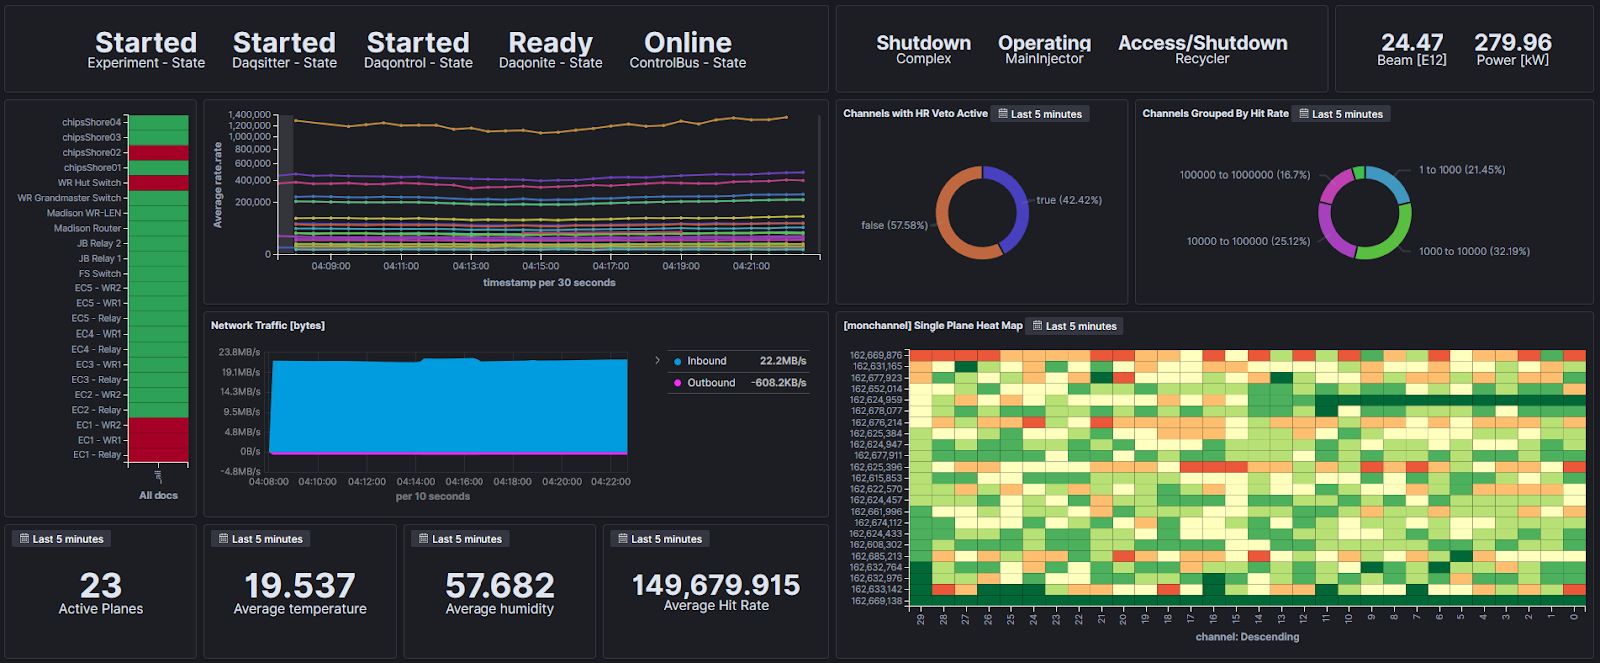
\includegraphics[width=\textwidth]{diagrams/5-daq/monitoring.png}
    \caption[monitoring short]
    {monitoring long}
    \label{fig:monitoring}
\end{figure}